%%%%%%%%%%%%%%%%%%%%
% hudba

\section{Hudba}

Pro přehrávání hudby v intru jsem použil knihovnu libv2 od německé skupiny Farbrausch \cite{V2}.
Ke knihovně je dodáván i příklad přehrávače souborů v2m.
Přehrávač byl napsán v jazyce C pro Visual Studio.
Některé části kódu byly napsány v jazyce assembler a ty bylo nutné přepsat.
Pro skládání hudby je ke knihovně přidán i VSTi plugin, zobrazen na obrázku \ref{fig:vsti}.
Hudbu jsem skládal v demo verzi programu FL Studio \cite{FLS} a použil jsem tento VSTi plugin.

\begin{figure}[h]
\centering
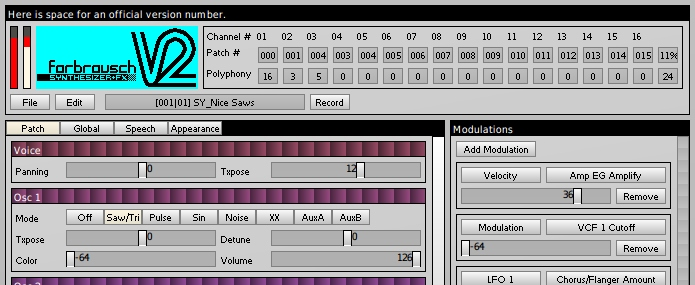
\includegraphics[width=15cm,keepaspectratio]{obr/vsti.jpg}
\caption{VSTi plugin pro tvorbu hudby pro knihovnu libv2.}
\label{fig:vsti}
\end{figure}

